\documentclass[UTF8]{article} % chinese
% \usepackage{ctex}
%\documentclass{article}     %english
%\usepackage[nonatbib]{neurips}
\usepackage[final]{aneurips}
\usepackage[utf8]{inputenc} % allow utf-8 input
\usepackage[T1]{fontenc}    % use 8-bit T1 fonts
\usepackage{hyperref}       % hyperlinks
\usepackage{url}            % simple URL typesetting
\usepackage{booktabs}       % professional-quality tables
\usepackage{amsfonts}       % blackboard math symbols
\usepackage{nicefrac}       % compact symbols for 1/2, etc.
\usepackage{microtype}      % microtypography
\usepackage{amsmath}
\usepackage{bm}
\usepackage{float}
\usepackage{enumitem}
\usepackage{multirow}
\usepackage{adjustbox}
\usepackage{color,xcolor,colortbl}
\usepackage{svg}
\usepackage[ruled, vlined, linesnumbered]{algorithm2e}
\newcommand{\mycomment}{\color{black}}
\newtheorem{lemma}{Lemma}
\newtheorem{theorem}{Theorem}
\graphicspath{{figure/}{images}}


\title{Paper Title}

\author{%
  Author First\thanks{corresponding author} \\
  Department of Computer \\
  Beijing University of Chemical Technology \\
  \texttt{first@mail.buct.edu.cn} \\
  \And
  Hao Li \\  
  Department of Computer \\
  Beijing University of Chemical Technology \\
  \texttt{2018040206@mail.buct.edu.cn} \\
}

\begin{document}

\maketitle

\begin{abstract}
Graph Neural Networks (GNN) is an emerging field for learning on non-Euclidean data. Recently, there has been great interest in designing GNN that scales to large graphs. Most existing techniques use ``graph sampling'' or ``layer-wise sampling'' technique to reduce training time. 

解决了什么问题?论文主要工作?效果如何?
~\\
~\\
~\\
\end{abstract}
\section{Method}

\begin{figure}[ht]
  \begin{center}
  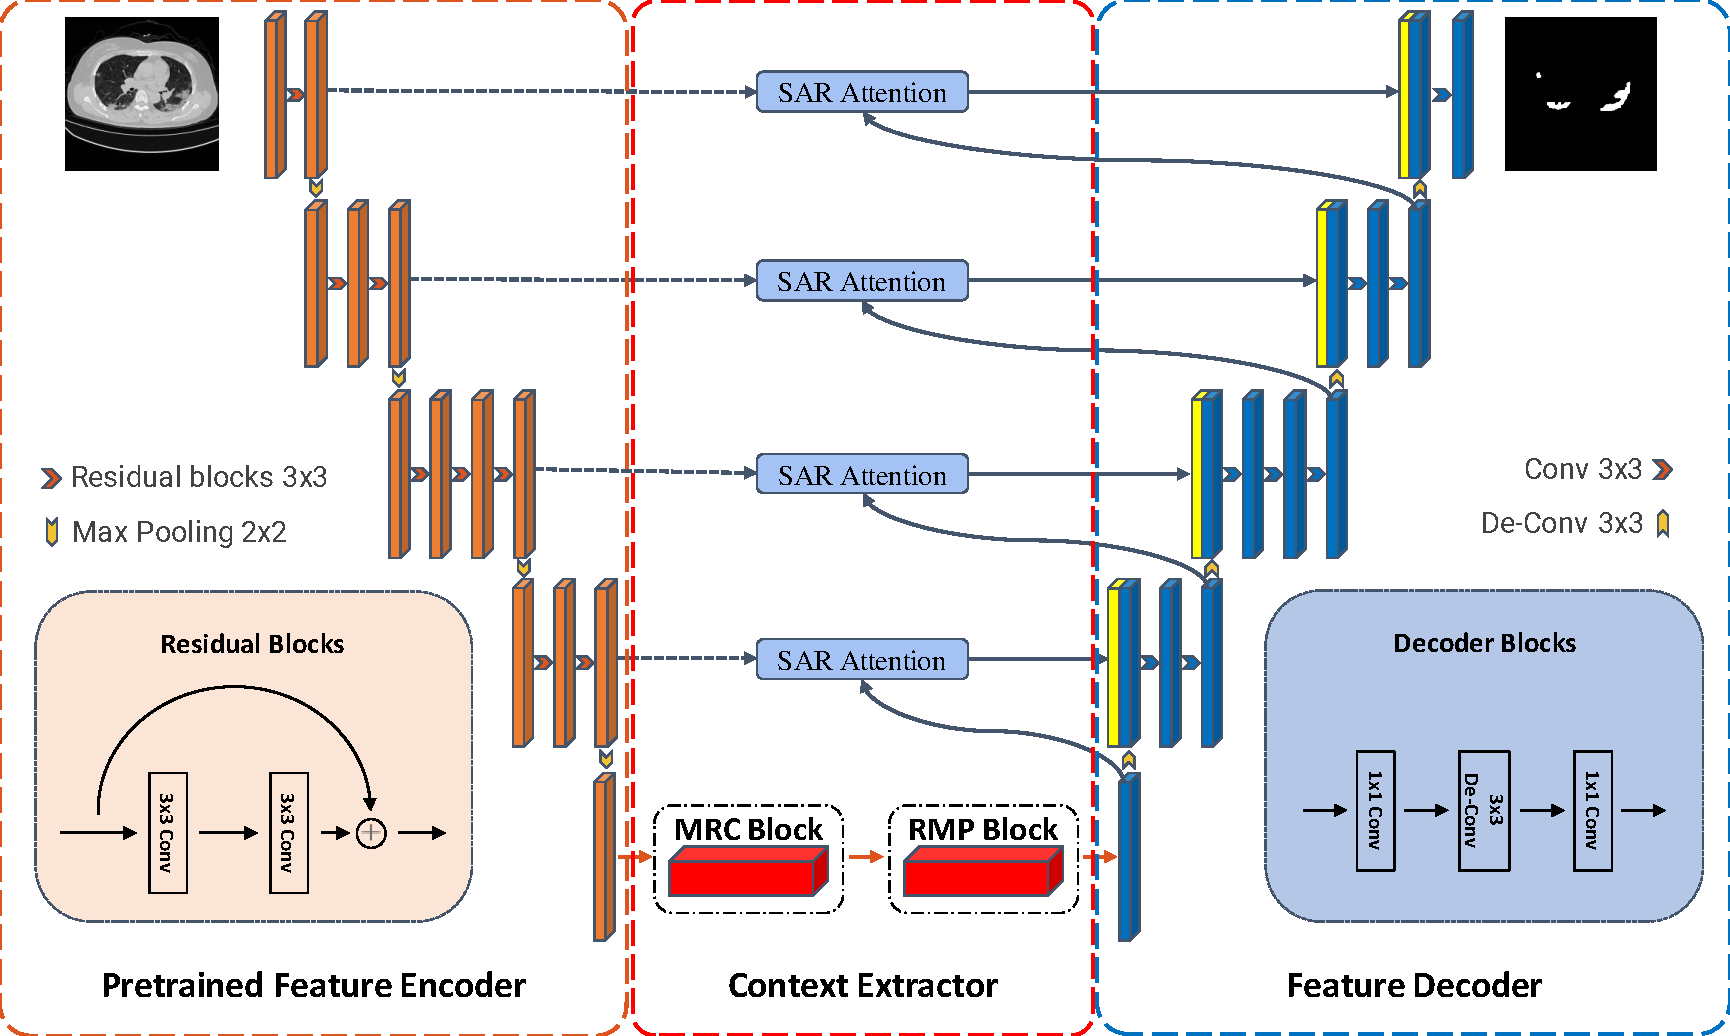
\includegraphics[width=0.9\textwidth]{overview.pdf}
  \vspace{-2mm}
  \caption{Illustration of our proposed network.} 
  \vspace{-2mm}
  \label{fig:overview}
  \end{center}
  \vspace{-0.35cm}
\end{figure}


\begin{figure}[htbp]
  \centering
  \begin{minipage}[t]{0.48\textwidth}
  \centering
  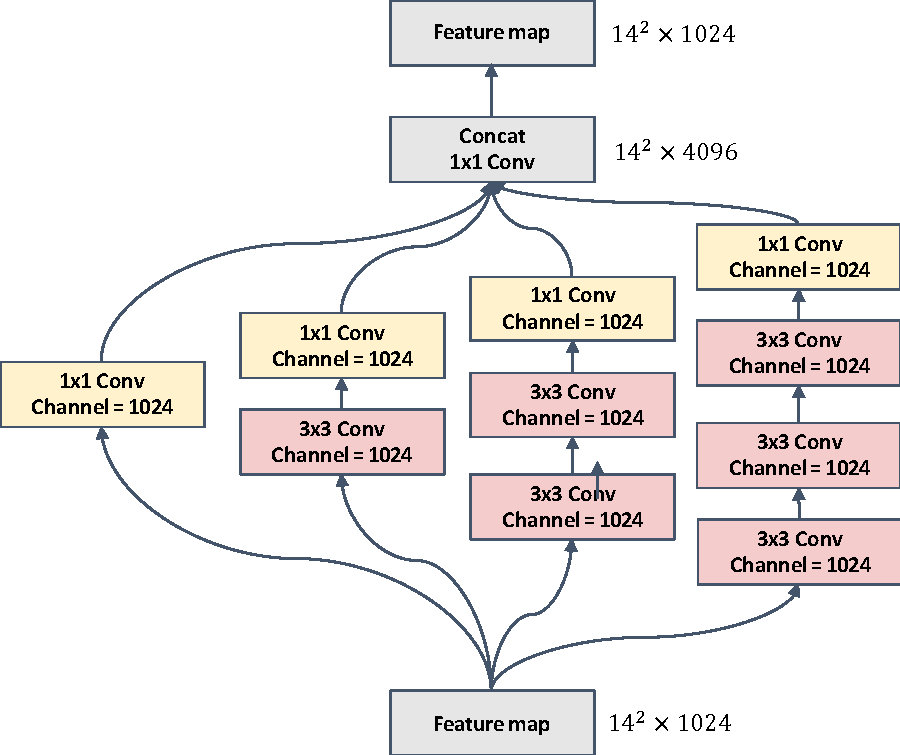
\includegraphics[width=0.9\textwidth]{DAC_block.pdf}
  \label{dac_block}
  \end{minipage}
  \begin{minipage}[t]{0.48\textwidth}
  \centering
  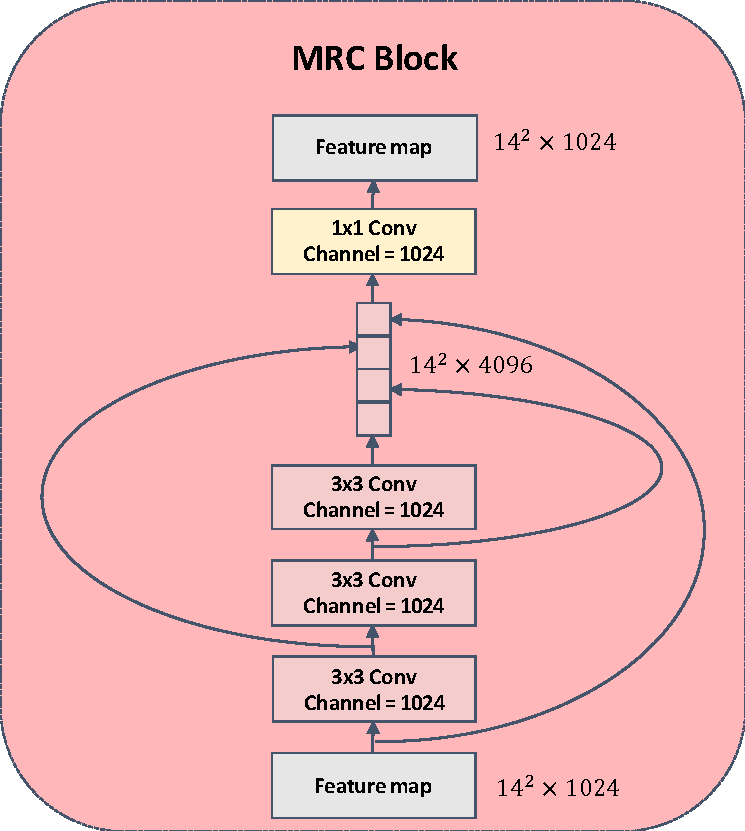
\includegraphics[width=0.9\textwidth]{MRC_block.pdf}
  \label{mrc_block}
  \end{minipage}
  \caption{(\ref{dac_block}) is the illustration of DAC Block. (\ref{mrc_block}) is the illustration of MRC Block.}
\end{figure}
  
\begin{figure}[ht]
  \begin{center}
  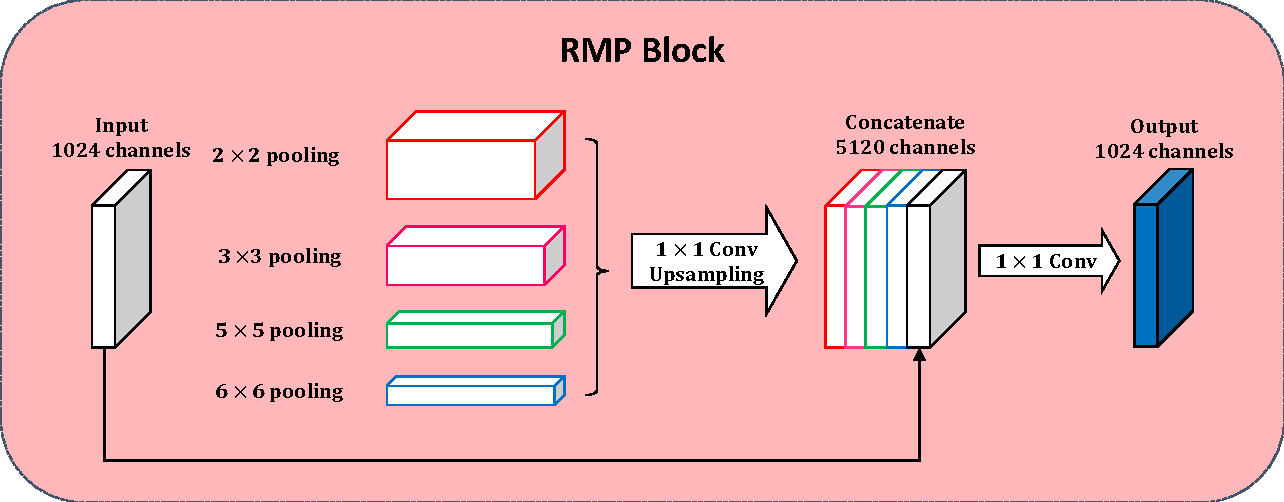
\includegraphics[width=0.6\textwidth]{rmp_block.pdf}
  \vspace{-2mm}
  \caption{Illustration of RMP Block.} 
  \vspace{-2mm}
  \label{fig:rmp_block}
  \end{center}
  \vspace{-0.35cm}
\end{figure}

\begin{figure}[ht]
  \begin{center}
  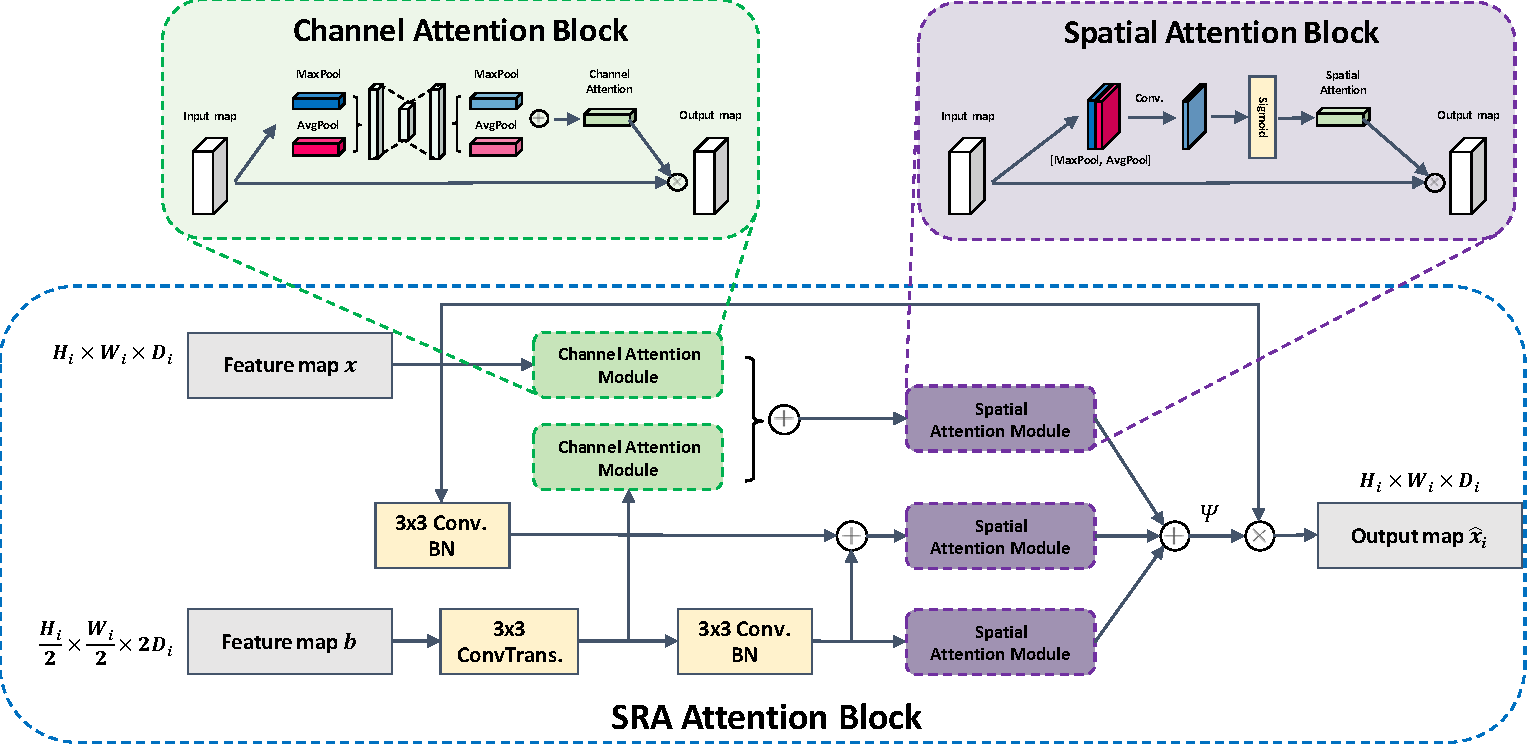
\includegraphics[width=0.9\textwidth]{Attention.pdf}
  \vspace{-2mm}
  \caption{Illustration of SRA Attention Block.} 
  \vspace{-2mm}
  \label{fig:Attention}
  \end{center}
  \vspace{-0.35cm}
\end{figure}

\begin{table}[H]
  \vspace{-2mm}
  \begin{center}\small
  \caption{Memorize Cost Comparison With Different Methods In Bottleneck}
  \label{param-table}
  \begin{tabular}{ccccccc}
    
  \toprule
  Backbone & Components & Params & Params size \\
  \midrule
    ResU-Net & SAR+DAC+RMP(CE-Net) & 135,571,137 & 517.16 \\
    ResU-Net & SAR+ASPP    & 92,573,377 & 353.14  \\
    ResU-Net & SAR+MRC+RMP & 94,669,505 & 361.14  \\
\bottomrule    
  \end{tabular}
  \end{center}
  %\vspace{-0.35cm}
  \vspace{-4mm}
\end{table}

\section{Experiments}
\subsection{Baseline and implementation}
We used a server equipped with an Intel Core i9-9980XE CPU @ 3.00GHz with 64GB RAM and 12GB of RTX2080Ti GPU for
our proposed networks training. The operating system of the sever is 64-bits Ubuntu 18.04. The structure of the network 
is implemented under the open source deep learning library Pytorch with VSCode implementation.

\subsection{Dataset}
For this study, we conduct our experiments on four differents segmentation tasks. 
Covering lesions/organs from most commonly used medical imaging modalities including microscopy, 
computed tomography (CT), and magnetic resonance imaging (MRI).  Table \ref{dataset-table} summarize those datasets in our study.

\begin{table}[ht]
  \vspace{-2mm}
  \begin{center}\small
  \caption{Summaey Of Biomedical Image Segmentation Datasets Used In Our Experiments}
  \label{dataset-table}
  \begin{tabular}{ccccc}
    
  \toprule
  Dataset & Image & Input Size & Modality & Provider\\
  \midrule
  Cell & 30 & $512\times 512$  & EM      & ISBI 2012\cite{isbicell}   \\
  Liver    & 4,000 & $512\times 512$       & CT     & MICCAI 2017 LiTS\cite{liver}  \\
  DSB2018      & 670 & $256\times 256$      & EM      & Kaggle\cite{dsb2018} \\
  COVID19         & 1,800 & $630\times 630$     & CT     & Web\cite{covid19,covid19_2}  \\
\bottomrule    
  \end{tabular}
  \end{center}
  %\vspace{-0.35cm}
  \vspace{-4mm}
  \end{table}

\paragraph{Cell}
The datset is the segmentation of neuronal structures in electron microscopic recordings.
The dataset is provided by the EM segmentation challenge\cite{isbicell} that is started at ISBI 2012.
The data is a set of 30 images ($512\times 512$ pixels) from serial section transmission electron
microscopy of the Drosophila first instar larva ventral nerve cord (VNC). Each image comes with a corresponding fully annotated ground truth segmentation
map for cells (white) and membranes (black).

\paragraph{Liver}
Liver tumor Segmentation Challenge (LiTS)\cite{liver} contain 131 contrast-enhanced CT images provided by hospital around the world with \(512 \times 512\) resolution.
The ground truth segmentation provides two different labels: liver and lesion. For our experiments,
we only consider liver as positive class and others as negative class.


\paragraph{COVID19}
Dataset\cite{covid19} includes whole volumes and includes, therefore, both positive and negative slices 
(373 out of the total of 829 slices have been evaluated by a radiologist as positive and segmented). 
Dataset\cite{covid19_2} contains 20 CT scans of patients diagnosed with COVID-19 as well as segmentations of lungs and infections made by experts.
These volumes are converted and normalized in a similar way as above, meanwhile we resize the data to $512\times 512$.

\subsection{Evaluation metrics}
The experiments are implemented using the Pytorch framework. We use Adam optimizer\cite{Adam} as our
models' optimizer with a learning rate of 0.00001, batch size of 2. All of datasets are splitted into training set and validation set with 
the ratio of 8:2 using sklearn library. To numerically evaluate, we use five widely adopted metrics, \(i.e.\),
the Dice similarity coefficient(Dice.), F1 score., Sensitivity(Sen.), Iou. and hausdorff distance(Hd)., the expressions of them are defined as follows:
\begin{align}
  \text { Sensitivity }=\frac{T P}{T P+F N}
\end{align}
\begin{align}
  \operatorname{DSC}(G, S)=\frac{2|G \cap S|}{|G|+|S|}
\end{align}
\begin{align}
  \operatorname{IOU}(G, S)=\frac{|G \cap S|}{|G| \cup|S|}
\end{align}
\begin{align}
  F_{1}=2 \cdot \frac{\text { precision } \cdot \text { recall }}{\text { precision }+\text { recall }}
\end{align}
\begin{align}
  h(G, S)=\max _{g \in G}\left\{\min _{c \in C}\|g-c\|\right\}
\end{align}
\subsection{Semantic Segmentation Results}
For comparsion, we use five origianl network FCN with 32s\cite{fcn}, U-Net\cite{unet}, U-Net++\cite{unet++} , CE-Net\cite{cenet} and U-Net with Attention Gate\cite{attentiongate}
to evaluate our proposaed method.
\begin{figure}[ht]
  \begin{center}
  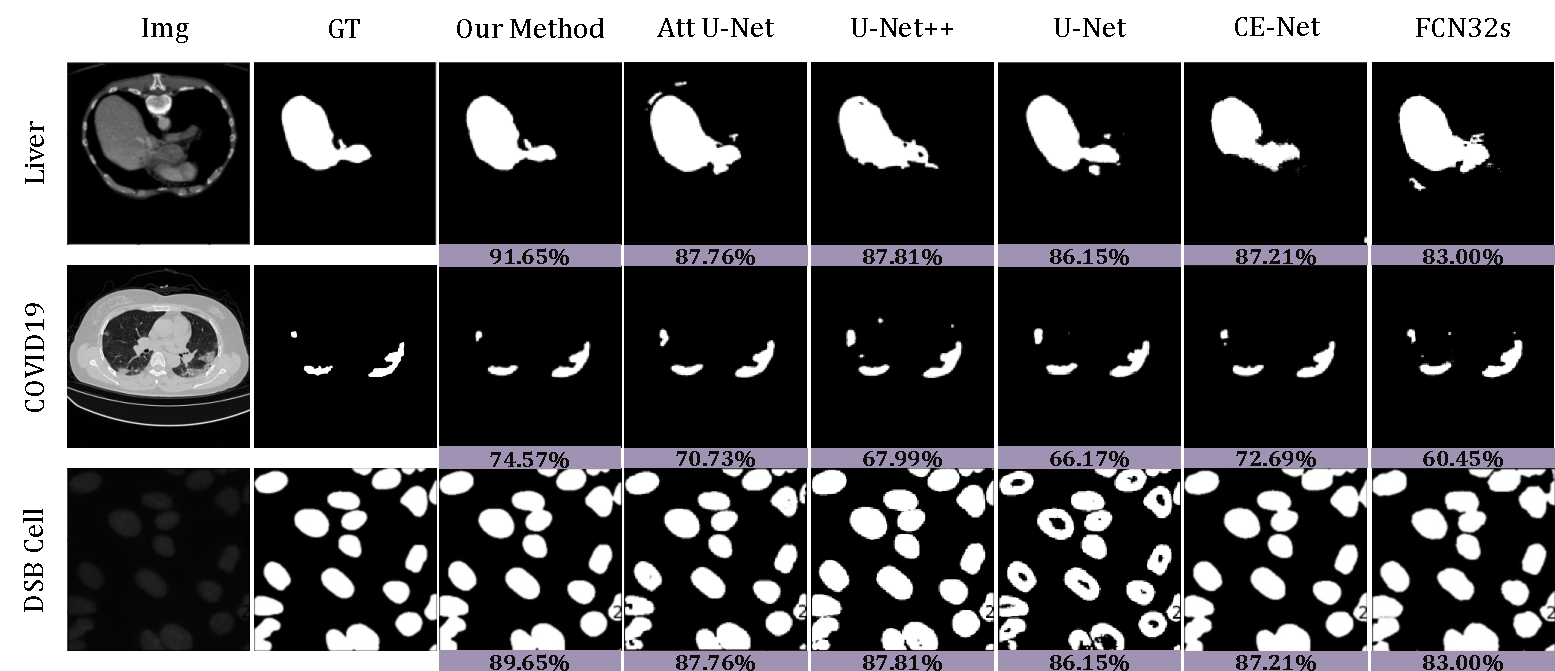
\includegraphics[width=0.99\textwidth]{result.pdf}
  \vspace{-2mm}
  \caption{Medical image segmentation examples.} 
  \vspace{-2mm}
  \label{fig:result}
  \end{center}
  \vspace{-0.35cm}
\end{figure}
\subsubsection{Performance in Cell segmentation task}
Segmentation results of cell segmentation are shown in table\ref{cell-table}, 

  \begin{table}[H]
    \vspace{-2mm}
    \begin{center}\small
    \caption{Comparsion With Other Methods In Cell\cite{dsb2018} Dataset}
    \label{cell-table}
    \begin{tabular}{ccccccc}
      
    \toprule
    Methods & Shape Loss & Dice. & F1 score. & Iou. & Sens. & Hd.\\
    \midrule
      Our proposal & $\surd$ & \textbf{0.8588} & \textbf{0.8588} & \textbf{0.7623} & \textbf{0.9296} & \textbf{4.6224}\\
      CENet & $\times$ & 0.8458 & 0.8458 & 0.7418 & 0.8316 & 5.2098\\
      UNet++ & $\times$ & 0.8439 & 0.8439 & 0.7396 & 0.8643 & 5.5307\\
      Attention UNet & $\times$ & 0.8153 & 0.8153 & 0.7015 & 0.8557 & 5.3695\\
      UNet  & $\times$  & 0.7977 & 0.7977 & 0.6893 & 0.8115 & 5.5049\\
      FCN32s & $\times$ & 0.6895 & 0.6895 & 0.5653 & 0.7760 & 7.1192\\
  \bottomrule    
    \end{tabular}
    \end{center}
    %\vspace{-0.35cm}
    \vspace{-4mm}
  \end{table}

  \subsubsection{Performance in liver segmentation task}
Segmentation results of cell segmentation are shown in table\ref{liver-table}, 

  \begin{table}[H]
    \vspace{-2mm}
    \begin{center}\small
    \caption{Comparsion With Other Methods In Liver\cite{liver} Dataset}
    \label{liver-table}
    \begin{tabular}{ccccccc}
      
    \toprule
    Methods & Shape Loss & Dice. & F1 score. & Iou. & Sens. & Hd.\\
    \midrule
     Our proposal & $\surd$ & \textbf{0.9551} & \textbf{0.9551} & \textbf{0.9165} & \textbf{0.9389} & \textbf{3.8854}\\
     U-Net++ & $\times$ & 0.9351 & 0.9351 & 0.8781 & 0.9156 & 5.8218\\
     Attention UNet & $\times$ & 0.9346 & 0.9346 & 0.8776 & 0.9056 & 4.836\\
     CENet & $\times$ & 0.9315 & 0.9315 & 0.8721 & 0.9045 & 4.904\\
     U-Net & $\times$ & 0.9253 & 0.9253 & 0.8615 & 0.9106 & 6.6785\\
     FCN32s & $\times$ & 0.9065 & 0.9065 & 0.8300 & 0.9381 & 7.97\\
  \bottomrule    
    \end{tabular}
    \end{center}
    \vspace{-4mm}
  \end{table}

  

  \subsubsection{Performance in covid19 lesion segmentation task}
  Segmentation results of cell segmentation are shown in table\ref{covid19-table}, 

  \begin{table}[H]
    \vspace{-2mm}
    \begin{center}\small
    \caption{Comparsion With Other Methods In COVID19\cite{covid19_2} Dataset}
    \label{covid19-table}
    \begin{tabular}{ccccccc}
      
    \toprule
    Methods & Shape Loss & Dice. & F1 score. & Iou. & Sens. & Hd.\\
    \midrule
      Our proposal & $\surd$ & \textbf{0.8489} & \textbf{0.8489} & \textbf{0.7457} & \textbf{0.8570} & \textbf{4.313}\\
      CENet & $\times$ & 0.8348 & 0.8348 & 0.7290 & 0.9359 & 4.7711\\
      UNet++ & $\times$ & 0.8014 & 0.8014 & 0.6799 & 0.9426 & 5.0301\\
      Attention UNet & $\times$ & 0.8229 & 0.8229 & 0.7073 & 0.9435 & 4.8845\\
      UNet  & $\times$ & 0.7874 & 0.7874 & 0.6617 & 0.9528 & 5.2231\\
      FCN32s & $\times$ & 0.7409 & 0.7409 & 0.6045 & 0.9935 & 5.8644\\
  \bottomrule    
    \end{tabular}
    \end{center}
    %\vspace{-0.35cm}
    \vspace{-4mm}
  \end{table}

  \subsubsection{Performance in lung segmentation task}
  Segmentation results of cell segmentation are shown in table\ref{lung-table}, 
    
  \begin{table}[H]
    \vspace{-2mm}
    \begin{center}\small
    \caption{Comparsion With Other Methods In Lung\cite{covid19_2} Dataset}
    \label{lung-table}
    \begin{tabular}{ccccccc}
      
    \toprule
    Methods & Shape Loss & Dice. & F1 score. & Iou. & Sens. & Hd.\\
    \midrule
      Our proposal & $\surd$ & \textbf{0.9392} & \textbf{0.9392} & \textbf{0.8965} & \textbf{0.9261} & \textbf{10.19714}\\
      UNet++ & $\times$ & 0.9351 & 0.9351 & 0.8781 & 0.9156 & 5.8218\\
      Attention UNet & $\times$ & 0.9346 & 0.9346 & 0.8776 & 0.9056 & 4.836\\
      CENet & $\times$ & 0.9315 & 0.9315 & 0.8721 & 0.9045 & 4.904\\
      UNet & $\times$ & 0.9253 & 0.9253 & 0.8615 & 0.9106 & 6.6785\\
      FCN32s & $\times$ & 0.9065 & 0.9065 & 0.8300 & 0.9381 & 7.97\\
  \bottomrule    
    \end{tabular}
    \end{center}
    %\vspace{-0.35cm}
    \vspace{-4mm}
  \end{table}
  


  \subsection{Ablation study}
  To justify the effectiveness of the pretrained U-Net\cite{unet}, Res-UNet\cite{ResUNet}, 
  MRC(multi residual convolution) block, RMP block and SAR(spatial channel and gateway) Attention block
  in our proposed method, we conduct the following ablation study using the COVID19 and Cell dataset as examples:


  \begin{table}[H]
    \vspace{-2mm}
    \begin{center}\small
    \caption{Comparsion With Other loss functions In COVID19\cite{covid19} Dataset}
    \label{loss-table}
    \begin{tabular}{ccccccc}
      
    \toprule
    Methods & Loss & Dice. & F1 score. & Iou. & Sens. & Hd.\\
    \midrule
      Our proposal & BCE          & 0.8076 & 0.8076 & 0.6874 & 0.8772 & 5.0112\\
      Our proposal & BCE+DiceLoss & 0.8375 & 0.8375 & 0.7282 & 0.8827 & 4.7241\\
      Our proposal & Ours         & 0.8489 & 0.8489 & 0.7457 & 0.8570 & 4.4313\\
  \bottomrule    
    \end{tabular}
    \end{center}
    %\vspace{-0.35cm}
    \vspace{-4mm}
  \end{table}

  \begin{table}[H]
    \vspace{-2mm}
    \begin{center}\small
    \caption{Ablation study for each component on COVID19 dataset}
    \label{loss-table}
    \begin{tabular}{ccccccc}
      
    \toprule
    Methods & Loss & Dice. & F1 score. & Iou. & Sens. & Hd.\\
    \midrule
      U-Net                & BCE & 0.7874 & 0.7874 & 0.6617 & 0.9528 & 5.2231\\
      ResU-Net             & BCE & 0.8105 & 0.8105 & 0.6923 & 0.9601 & 5.0248\\
      ResU-Net + MRC + RMP & BCE & 0.8185 & 0.8185 & 0.7030 & 0.9295 & 4.8931\\
      ResU-Net + SAR       & BCE & 0.7988 & 0.7988 & 0.6846 & 0.7969 & 5.1522\\  % trick
      ResU-Net+SAR+MRC+RMP & BCE & 0.8076 & 0.8076 & 0.6874 & 0.8772 & 5.0112\\
      ResU-Net+SAR+MRC+RMP & Ours & \textbf{0.8489} & \textbf{0.8489} & \textbf{0.7457} & \textbf{0.8570} & \textbf{4.313}\\
  \bottomrule    
    \end{tabular}
    \end{center}
    %\vspace{-0.35cm}
    \vspace{-4mm}
  \end{table}

  \begin{figure}[ht]
    \begin{center}
    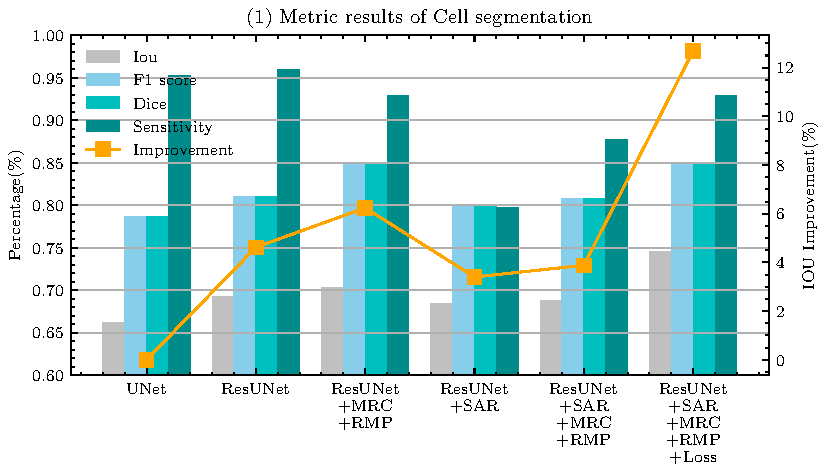
\includegraphics[width=0.6\textwidth]{covid_comparison.pdf}
    \vspace{-2mm}
    \caption{Fig 1 shows ; Fig 2 shows; Fig 3 shows; Fig 4 shows;Fig5 shows.} 
    \vspace{-2mm}
    \label{fig:covid_comparison}
    \end{center}
    \vspace{-0.35cm}
  \end{figure}

  \begin{table}[H]
    \vspace{-2mm}
    \begin{center}\small
    \caption{Ablation study for each component on Cell dataset}
    \label{loss-table}
    \begin{tabular}{ccccccc}
      
    \toprule
    Methods & Loss & Dice. & F1 score. & Iou. & Sens. & Hd.\\
    \midrule
      U-Net                & BCE & 0.7977 & 0.7977 & 0.6893 & 0.8115 & 5.5049\\
      ResU-Net             & BCE & 0.8314 & 0.8314 & 0.7274 & 0.9685 & 5.5861\\
      % ResU-Net+CBAM\cite{cbam}& BCE &  &  &  &  & \\
      ResU-Net + MRC + RMP & BCE & 0.8448 & 0.8448 & 0.7414 & 0.9714 & 5.0647\\
      ResU-Net + SAR       & BCE & 0.8545 & 0.8545 & 0.7534 & 0.9669 & 4.9601\\
      ResU-Net+SAR+MRC+RMP & BCE & 0.8525 & 0.8525 & 0.7598 & 0.9744 & 4.9210\\
      ResU-Net+SAR+MRC+RMP & Ours & \textbf{0.8588} & \textbf{0.8588} & \textbf{0.7623} & \textbf{0.9296} & \textbf{4.6224}\\
  \bottomrule    
    \end{tabular}
    \end{center}
    %\vspace{-0.35cm}
    \vspace{-4mm}
  \end{table}

  \begin{figure}[ht]
    \begin{center}
    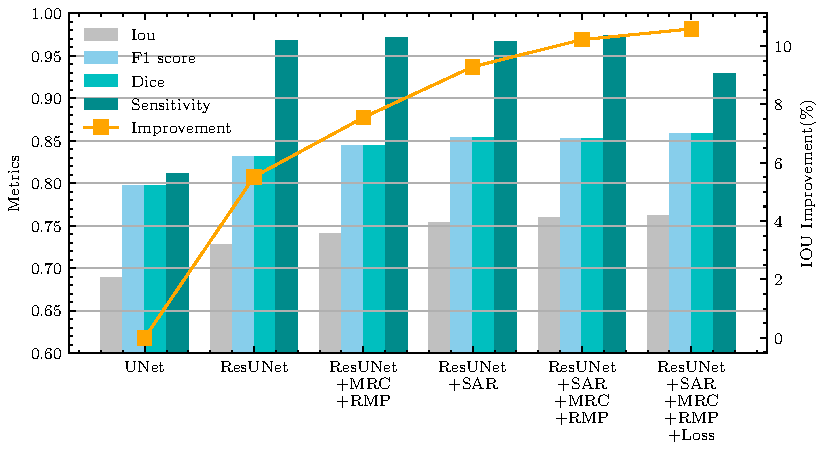
\includegraphics[width=0.6\textwidth]{cell_comparison.pdf}
    \vspace{-2mm}
    \caption{Fig 1 shows ; Fig 2 shows; Fig 3 shows; Fig 4 shows;Fig5 shows.} 
    \vspace{-2mm}
    \label{fig:cell_comparison}
    \end{center}
    \vspace{-0.35cm}
  \end{figure}
\section{Conclusion}
~\\
~\\
~\\

\section*{Acknowledgments}
~\\
~\\
~\\

\bibliographystyle{abbrv}
\bibliography{complete.bib}
\end{document}
